\section{Hybrid Metaheuristc}


A large  number of researchers have recognized the advantages and huge potential building
hybrid mathematical programming methods and metaheuristics.
The main motivation to create hybrid Metaheuristics is to exploit the complementary character of different optimization strategies. In fact, choosing an adequate combination of algorithmic can be the key for achieving top performance in solving many hard optimization problems \cite{Puchinger2005} \cite{Blum2012}.


There are two main categories of metaheuristc combinations: Collaborative Combinations and Integrative Combinations. The Fig. \ref{fig:metaheuristc} presents the two main categories of Hybrid MetaHeuristc \cite{Puchinger2005}.

\begin{figure}[h]
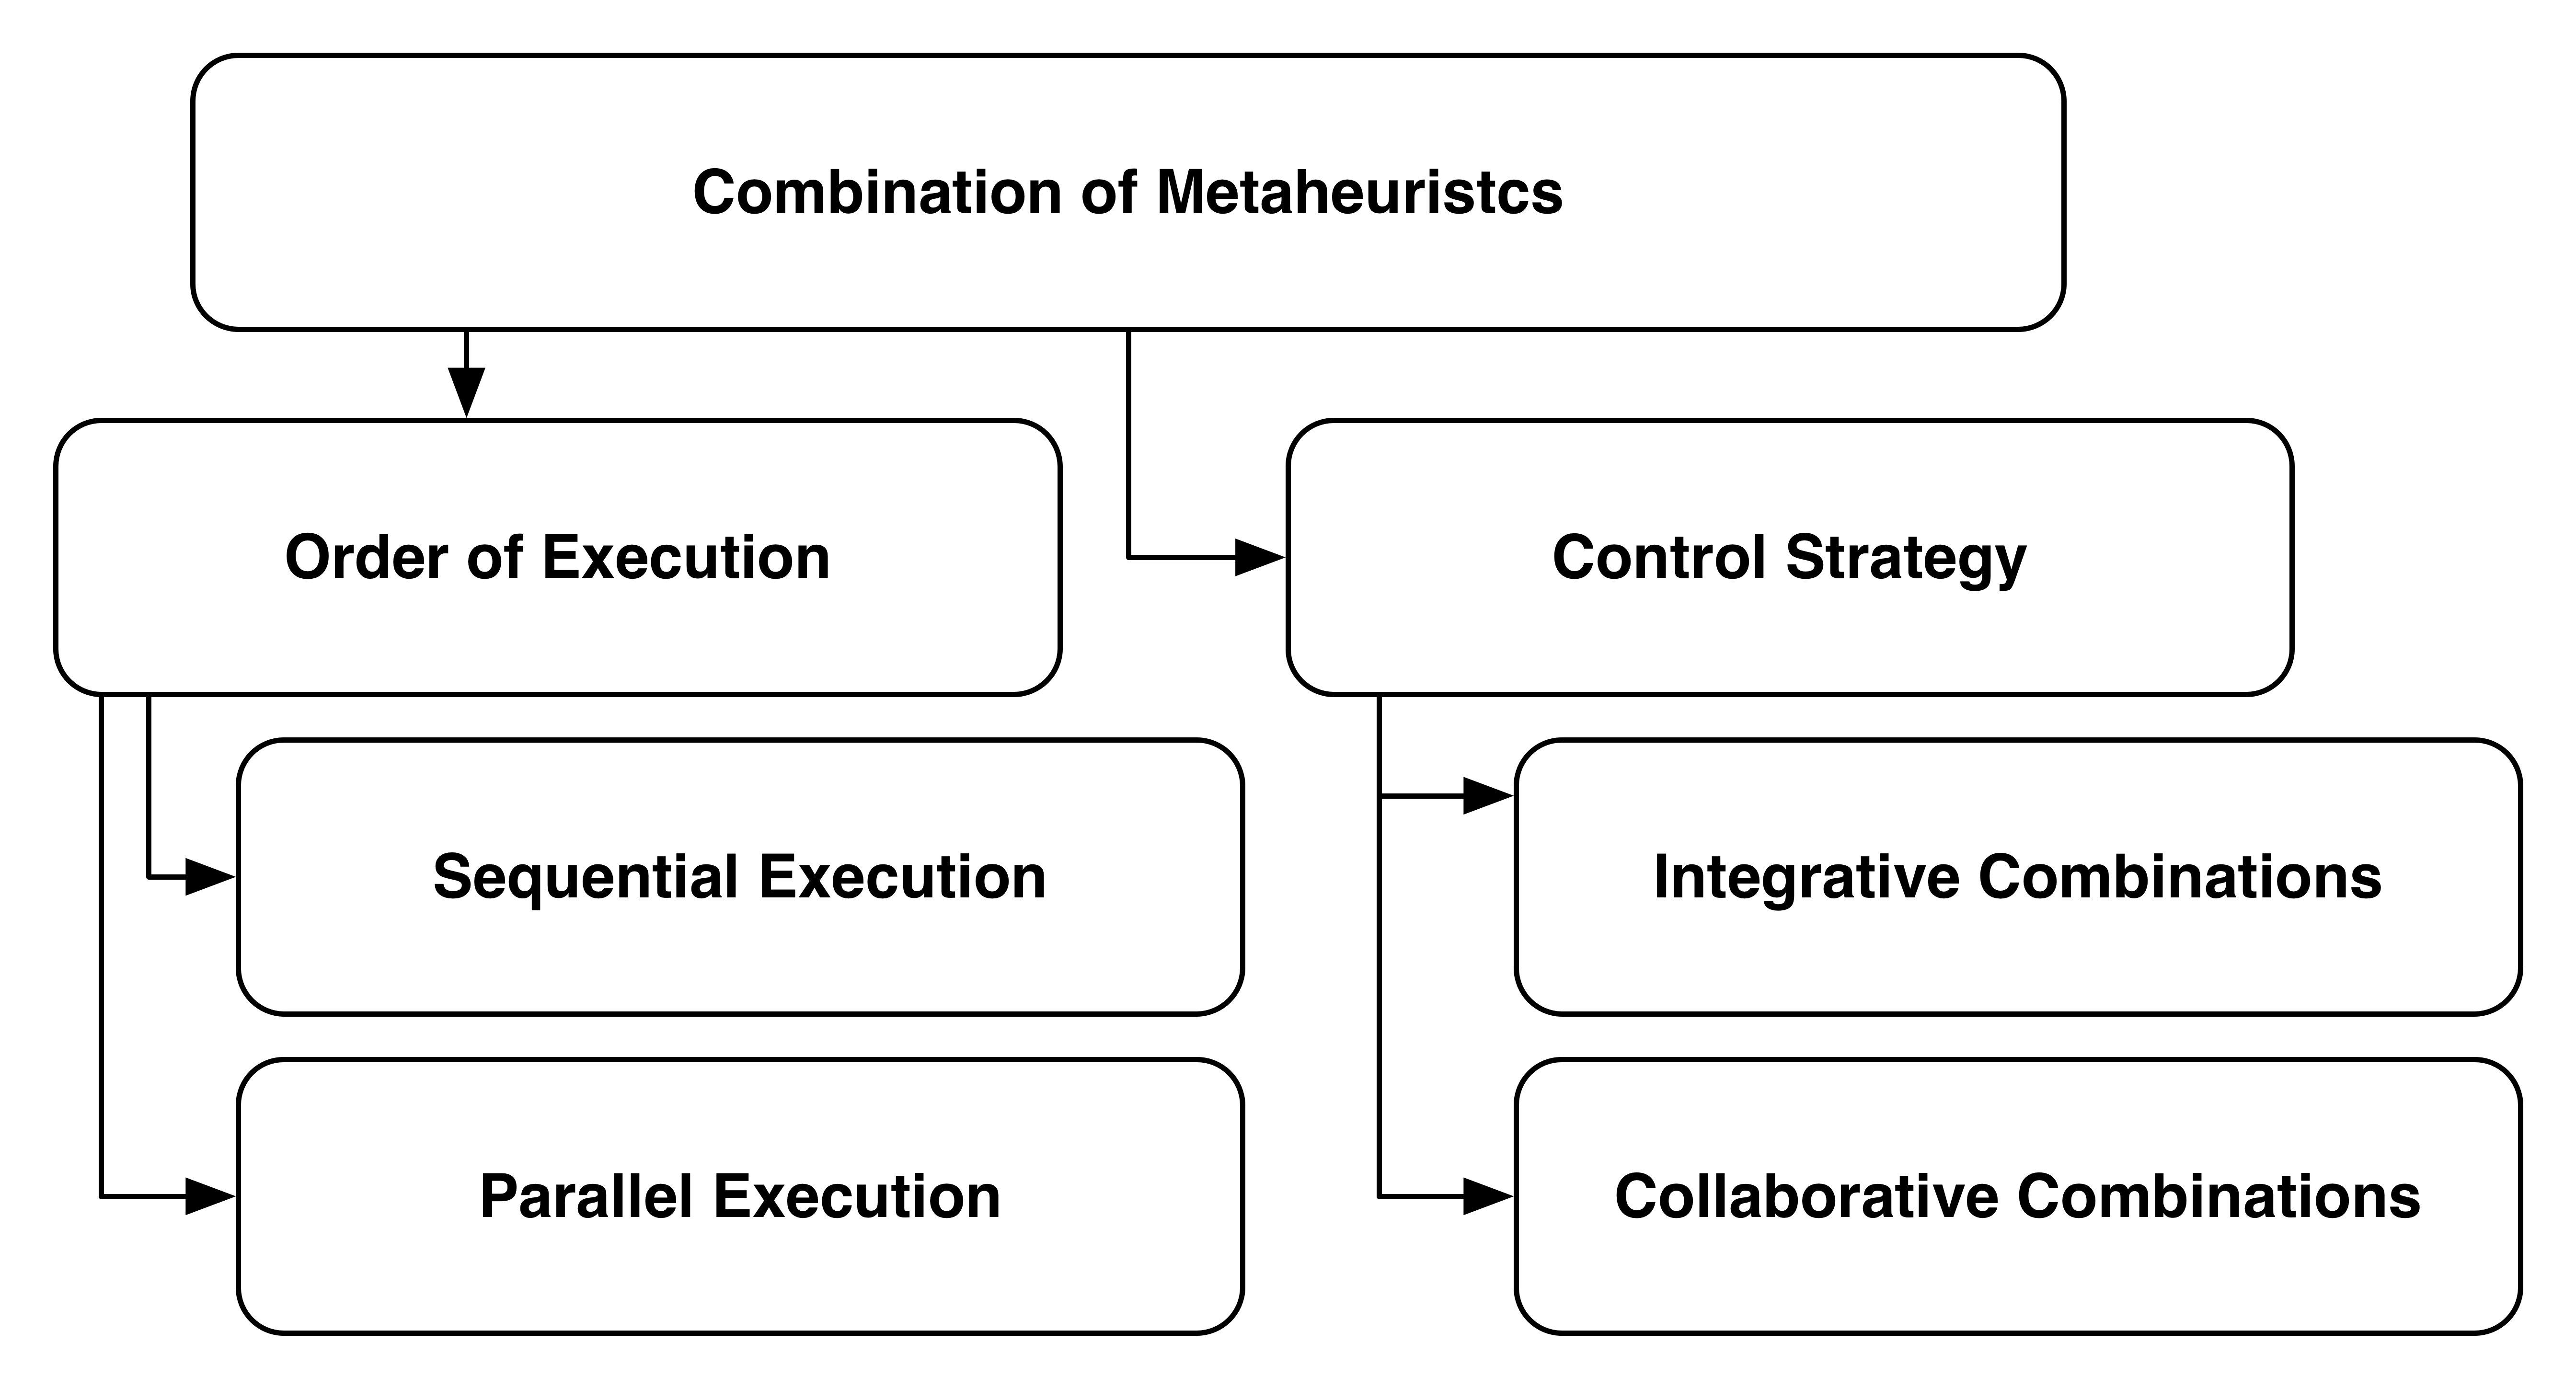
\includegraphics[width=0.5\textwidth]{./images/metaheuristc2.png}
\caption{Categories of metaheuristc combinations \cite{Puchinger2005} }
\label{fig:metaheuristc}
\end{figure}

Collaborative Combinations uses a approach where the  algorithms exchange information, but are not part of each other. In this approach,  algorithms may be executed sequentially or in parallel. The presented research work uses a type of  Collaborative Combination with Sequential Execution.

